\textbf{Ejemplo 6}\\
Dada la tasa de 2\% periódica mes vencido, hallar la tasa nominal anual trimestral vencida equivalente.\\

%\newpage %USAR SOLO SI EL SOLUCIÓN QUEDA SOLO Y ES NECESARIO BAJARLO A LA SIGUIENTE PAGINA
\textbf{Solución.}\\
%La tabla ira centrada
\begin{center}
  \renewcommand{\arraystretch}{1.5}% Margenes de las celdas
  %Creación de la cuadricula de 3 columnas
  \begin{longtable}[H]{|C{0.3\linewidth}|C{0.3\linewidth}|C{0.3\linewidth}|}
    %Creamos una linea horizontal
    \hline
    %Definimos el color de la primera fila
    \rowcolor[HTML]{FFB183}
    %%%%% INICIO ASIGNACIÓN PERíODO FOCAL %%%%%%%
    %%%%%%%%%% INICIO TITULO
    %Lo que se hace aquí es mezclar las 3 columnas en una sola
    \rowcolor[HTML]{FFB183}
    \multicolumn{3}{|c|}{\cellcolor[HTML]{FFB183}\textbf{1. Asignación período focal}}                                                                                                 \\ \hline
    \multicolumn{3}{|c|}{$pf: \textit{No aplica}$}                                                                                                                                     \\ \hline
    %%%%%%%%%% FIN TITULO
    %%%%% INICIO DECLARACIÓN DE VARIABLES %%%%%%%
    %%%%%%%%%% INICIO TITULO
    %Lo que se hace aquí es mezclar las 3 columnas en una sola
    \multicolumn{3}{|c|}{\cellcolor[HTML]{FFB183}\textbf{2. Declaración de variables}}                                                                                                 \\ \hline
    %%%%%%%%%% FIN TITULO
    %%%%%%%%%% INICIO SUBTITULO
    \cellcolor[HTML]{FFB183}\textbf{Valores monetarios}    & 
    \cellcolor[HTML]{FFB183}\textbf{Valores no monetarios} &
    \cellcolor[HTML]{FFB183}\textbf{Incógnitas}  \\ \hline
    %%%%%%%%%% FIN SUBTITULO
    %%%%%%%%%% INICIO DE MATEMÁTICAS
    %Cada & hace referencia al paso de la siguiente columna
    & $i_{1} = 2\% \textit{ pmv}$ & $j_{2} = ? \% \textit{ natv} $ \\
    & $m_{1} = 12 \textit{ pmv}$ & \\
    & $m_{2} = 4 \textit{ ptv}$ & \\ \hline       

    %%%%%%%%%% FIN DE MATEMÁTICAS
    %%%%% FIN DECLARACIÓN DE VARIABLES


    %%%%% INICIO FLUJO DE CAJA
    \rowcolor[HTML]{FFB183}
    \multicolumn{3}{|c|}{\cellcolor[HTML]{FFB183}\textbf{3. Diagrama de equivalencia de tasas}}                                                                                        \\ \hline
    %Mezclamos 3 columnas y pondremos el dibujo
    %%%%%%%%%%%%% INSERCIÓN DE LA IMAGEN
    %Deberán descargar las imágenes respectivas del drive y pegarlas en la carpeta
    %n_capitulo/img/ejemplos/1/capitulo1ejemplo1.pdf  (el /1/ es el numero del ejemplo)
    \multicolumn{3}{|c|}{ 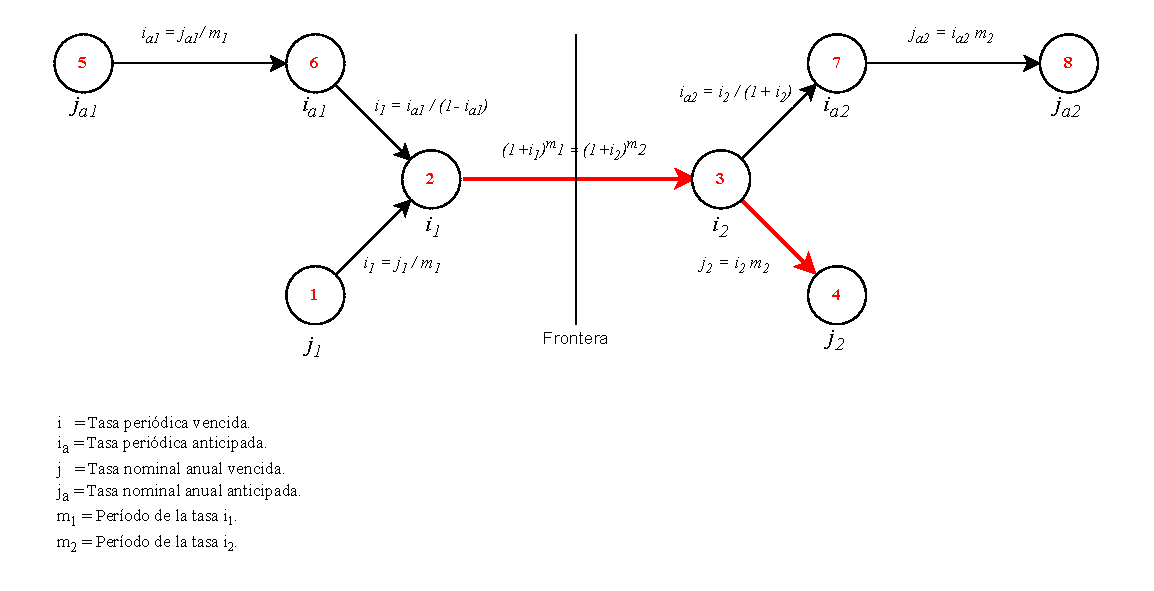
\includegraphics[height = 7.0 cm]{2_Capitulo/ejemplos/6/Capitulo2Ejercicio6.pdf} } \\ \hline

    %%%%%%%%%%%%% FIN INSERCIÓN DE IMAGEN
    %%%%%FIN FLUJO DE CAJA

    %%%%% INICIO DECLARACIÓN FORMULAS
    %%%%%%%%%%% INICIO TITULO
    \rowcolor[HTML]{FFB183}
    \multicolumn{3}{|c|}{\cellcolor[HTML]{FFB183}\textbf{4. Declaración de fórmulas}}                                                                                                  \\ \hline
    %%%%%%%%%%% FIN TITULO
    %%%%%%%%%%% INICIO MATEMÁTICAS

    \multicolumn{3}{|c|}{$(1+i_{1})^{m_1} = (1+i_{2})^{m_2}\hspace{0.3cm} \textit{Equivalencia de tasas}$}                  \\
    \multicolumn{3}{|c|}{$j=i(m)\hspace{0.3cm} \textit{Tasa periódica anualizada}$}
    \\ \hline 
    %%%%%%%%%% FIN MATEMÁTICAS
    %%%%%% INICIO DESARROLLO MATEMÁTICO
    \rowcolor[HTML]{FFB183}
    %%%%%%%%%%INICIO TITULO
    \multicolumn{3}{|c|}{\cellcolor[HTML]{FFB183}\textbf{5. Desarrollo matemático}}                                                                                                    \\ \hline
    %%%%%%%%%% FIN TITULO
    %%%%%%%%%% INICIO MATEMÁTICAS
    \multicolumn{3}{|c|}{$(1 + 0,020)^{12}= (1 + i_{2})^{4}$} \\
    \multicolumn{3}{|c|}{$(1,020)^\frac{12}{4}-1 = i_{2}$} \\
    \multicolumn{3}{|c|}{$i_{2}=0,0612 \textit{ ptv} \equiv$  $6,12\% \textit{ ptv}$} \\
    \multicolumn{3}{|c|}{$j_{2}=6,12\% \textit{ ptv}(4\textit{ ptv}$)} \\ 
    \multicolumn{3}{|c|}{$j_{2} = 24,4832\% \textit{ natv}$} \\ \hline
    %%%%%%%%%% FIN MATEMÁTICAS
    %%%%%% FIN DESARROLLO MATEMÁTICO
    %%%%%% INICIO RESPUESTA
    \rowcolor[HTML]{FFB183}
    %%%%%%%%%%INICIO TITULO
    \multicolumn{3}{|c|}{\cellcolor[HTML]{FFB183}\textbf{6. Respuesta}}                                                                                                                \\ \hline
    %%%%%%%%%% FIN TITULO
    %%%%%%%%%% INICIO RESPUESTA MATEMÁTICA
    \multicolumn{3}{|c|}{${j_{2} = 24,4832\%  \textit{ natv}}$} \\ \hline

    %%%%%%%%%% FIN MATEMÁTICAS
    %%%%%% FIN RESPUESTA
  \end{longtable}
  %Se crean dos lineas en blanco para que no quede el siguiente texto tan pegado
  %\newline \newline %USARLO SI CREES QUE ES NECESARIO
\end{center}
